\documentclass{udpreport}
%\headertext{Metodos Numéricos}
\title{Metodos Numéricos : Tarea 1}
\author{Thomas Muñoz , Diego Vilches , Javiera Araya , Ignacio Yanjari.}
\usepackage{amssymb}
\usepackage{amsmath}
\usepackage{graphicx}
\usepackage{float}
\usepackage{array}
\graphicspath{ {Imagenes/} }
\usepackage{listings}
\usepackage{color}

\definecolor{dkgreen}{rgb}{0,0.6,0}
\definecolor{gray}{rgb}{0.5,0.5,0.5}
\definecolor{mauve}{rgb}{0.58,0,0.82}

\lstset{frame=tb,
  language=MATLAB,
  aboveskip=3mm,
  belowskip=3mm,
  showstringspaces=false,
  columns=flexible,
  basicstyle={\small\ttfamily},
  numbers=none,
  numberstyle=\tiny\color{gray},
  keywordstyle=\color{blue},
  commentstyle=\color{dkgreen},
  stringstyle=\color{mauve},
  breaklines=true,
  breakatwhitespace=true,
  tabsize=4
}

\begin{document}
\maketitle
\tableofcontents
\listoffigures
\chapter{Introducción}

\chapter{Resolución de sistema de ecuaciones lineales} % rellenar con lo que corresponda
 \section{Programación}
 
 \section{Aplicación de los esquemas programados}
 \begin{enumerate}
 %%%%%%%%%%%%%%%
 %pregunta 1
 %%%%%%%%%%%%%%%%
 	\item   
 		\begin{enumerate}
 			\item 	
 			\begin{figure}[H]
 				\centering
 				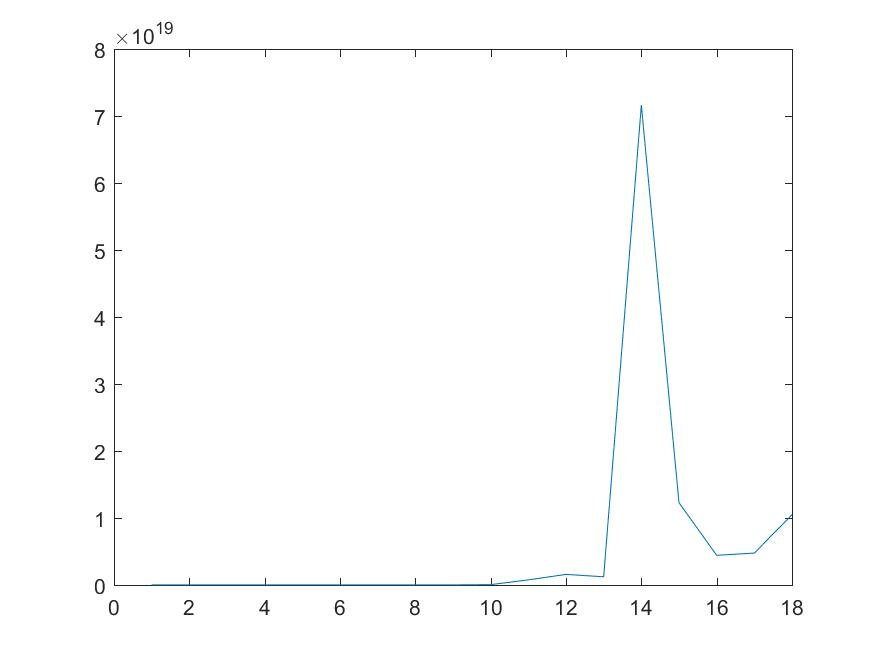
\includegraphics[width=9cm]{grafo1-a}
 				\caption{Gráfico del número de condición para una matriz de Hilbert de tamaño n}
 			\end{figure}
 			Se puede observar que entre más grande es el tamaño de la matriz de Hilbert, más grande es su número de condición. Este, al estar significativamente alejado del 1, implica que la matriz está mal condicionada.  %explica que significa que esté mal condicionada
 			\item 
 				\begin{itemize} 				
 				\item Para n=6:
 				
 				$x_{a} = \left(\begin{array}{c} 1.0\\ 1.0\\ 1.0\\ 1.0\\ 1.0\\ 1.0\\ \end{array}\right)$
 				\\
 				\\
 				\item Para n=10:
 				
 				$x_{a} = \left(\begin{array}{c} 1.0\\ 1.0\\ 1.0\\ 1.0\\ 1.0\\ 1.0\\ 0.9998\\ 1.0\\ 0.9999\\ 1.0 \end{array}\right)$
 				\\
 				\\
 				\item Para n=20:
 				
 				$x_{a} = \left(\begin{array}{c} 1.0\\ 1.0\\ 0.9992\\ 1.008\\ 0.9865\\ 0.6493\\ 4.094\\ -11.3\\ 28.09\\ -30.78\\ 14.27\\ 5.74\\ 8.759\\ -22.04\\ 9.068\\ 0.1336\\ 29.05\\ -42.82\\ 26.48\\ -4.379 \end{array}\right)$
 				\\
 				\\
 				\item Para n=30:
 				
 				$x_{a} = \left(\begin{array}{c} 1.0\\ 1.0\\ 1.0\\ 0.9929\\ 1.055\\ 0.7579\\ 1.695\\ -0.8953\\ 7.118\\ -14.6\\ 22.59\\ -5.381\\ -19.13\\ 19.89\\ 11.04\\ -26.6\\ 29.17\\ -27.26\\ 32.59\\ -26.64\\ 8.374\\ -8.23\\ 29.33\\ 9.701\\ -39.71\\ -9.034\\ 39.38\\ 2.024\\ -19.37\\ 8.151 \end{array}\right)$
 			\end{itemize}
 			\item 
 			\begin{figure}[H]
 				\centering
 				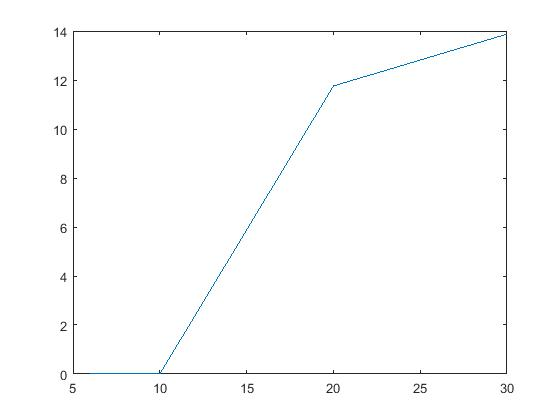
\includegraphics[width=9cm]{grafo1-rfe}
 				\caption{Gráfico del error relativo $rfe$}	
 			\end{figure}
 			
 			\begin{figure}[H]
 				\centering
 				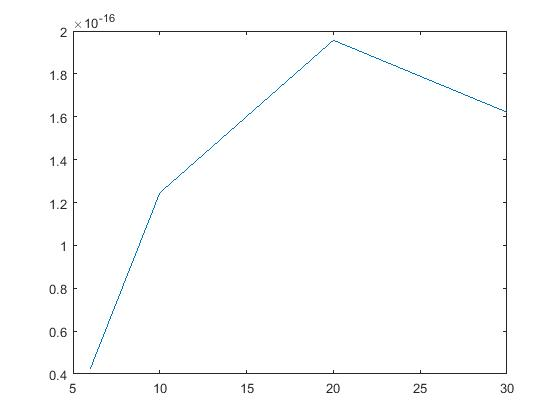
\includegraphics[width=9cm]{grafo1-rbe}
 				\caption{Gráfico del error relativo $rfb$}		
 			\end{figure}
 			
 			\begin{figure}[H]
 				\centering
 				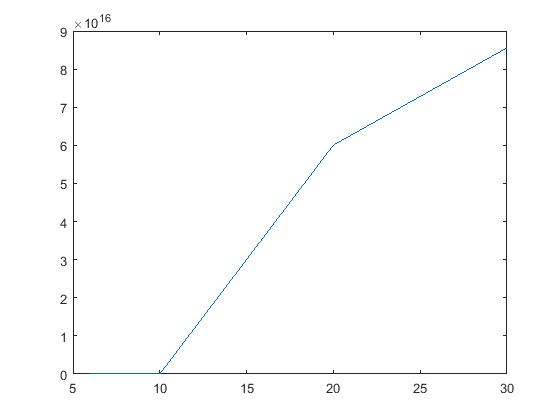
\includegraphics[width=9cm]{grafo1-div}
 				\caption{Gráfico de$\frac{rfe}{rbe}$}
	
 			\end{figure}
 		
 			En el primer gráfico se puede observar que para matrices de menor tamaño, el error es despreciable, pero a medida que el tamaño de la matriz aumenta también lo hace su error. Esto se produce debido al mal condicionamiento de la matriz de Hilbert.
 		\end{enumerate}
 		
 	Para resolver este problema se ocuparon los siguientes archivos: SolLU.m, FactorizacionLU.m, DiagUp.m y DiagDown.m	
 	 %%%%%%%%%%%%%%%
 %pregunta 6
 %%%%%%%%%%%%%%%%	
	\item
 		\begin{enumerate}
			\item 
			\item 	
			\begin{itemize}
				\item Cuando se ocupa el método de Richardson, este no converge para ninguno de los tres casos, ya que los valores del radio espectral de la matriz definida por $I-A$ son mayores a 1. Teniendo valores de 2.9854, 2.9962, 2.9973 para $n=25, n=50$ y $n=60$ respectivamente.
				
				\item Al ocupar el método de Jacobi, se obtienen los siguientes valores para:
				\begin{itemize}
					\item n=25: 
					
					$x_{a} = \left(\begin{array}{c} 0.03939\\ 0.07875\\ 0.1181\\ 0.1574\\ 0.1967\\ 0.2358\\ 0.275\\ 0.314\\ 0.353\\ 0.3917\\ 0.4305\\ 0.4691\\ 0.5077\\ 0.546\\ 0.5844\\ 0.6225\\ 0.6606\\ 0.6986\\ 0.7365\\ 0.7743\\ 0.8121\\ 0.8497\\ 0.8873\\ 0.9249\\ 0.9625 \end{array}\right) $
					
					
					\item n=50:
					
					$x_{a} = \left(\begin{array}{c} 0.0215\\ 0.04301\\ 0.06448\\ 0.08595\\ 0.1074\\ 0.1288\\ 0.1501\\ 0.1715\\ 0.1927\\ 0.2139\\ 0.235\\ 0.2561\\ 0.277\\ 0.2979\\ 0.3187\\ 0.3394\\ 0.36\\ 0.3805\\ 0.4009\\ 0.4212\\ 0.4414\\ 0.4615\\ 0.4814\\ 0.5013\\ 0.521\\ 0.5406\\ 0.5601\\ 0.5795\\ 0.5987\\ 0.6179\\ 0.6369\\ 0.6558\\ 0.6746\\ 0.6934\\ 0.7119\\ 0.7305\\ 0.7489\\ 0.7672\\ 0.7854\\ 0.8036\\ 0.8217\\ 0.8398\\ 0.8577\\ 0.8756\\ 0.8935\\ 0.9113\\ 0.9291\\ 0.9468\\ 0.9646\\ 0.9823 \end{array}\right)$
					
					\item n=60:
					
					$x_{a} = \left(\begin{array}{c} 0.0187\\ 0.03739\\ 0.05608\\ 0.07474\\ 0.09339\\ 0.112\\ 0.1306\\ 0.1491\\ 0.1676\\ 0.186\\ 0.2044\\ 0.2227\\ 0.2409\\ 0.2591\\ 0.2772\\ 0.2952\\ 0.3131\\ 0.3309\\ 0.3487\\ 0.3663\\ 0.3838\\ 0.4012\\ 0.4186\\ 0.4357\\ 0.4529\\ 0.4698\\ 0.4867\\ 0.5034\\ 0.5201\\ 0.5366\\ 0.553\\ 0.5692\\ 0.5854\\ 0.6014\\ 0.6174\\ 0.6332\\ 0.6489\\ 0.6644\\ 0.6799\\ 0.6953\\ 0.7106\\ 0.7257\\ 0.7408\\ 0.7557\\ 0.7706\\ 0.7853\\ 0.8001\\ 0.8147\\ 0.8293\\ 0.8437\\ 0.8581\\ 0.8725\\ 0.8868\\ 0.901\\ 0.9153\\ 0.9294\\ 0.9436\\ 0.9577\\ 0.9718\\ 0.9859 \end{array}\right)$
				\end{itemize}
			\end{itemize}
		\end{enumerate}
 		
 \end{enumerate}
\newpage
\chapter{Algo 2}
    

     
 \newpage

    
    
\chapter{Conclusión}
      

\end{document}
